%!TEX root = ../my_thesis.tex
\chapter{Techniques for fast z feedback}

Implementing model based controllers or high frequency actuators improves the AFM feedback loop\cite{sulchek1999dual}. The drawback with these actuators is the decrease in the positioning range.

We will improve the bandwidth and the scan range of our device. Past research has introduced an external piezoelectrical actuator on top of the cantilever. With this scheme, we can combine the advantages of a high bandwidth from the piezoelectrical actuator and the long range of the tip.

\section{Dual actuators system}
\label{sec:dualactuator}
The principal feature of an AFM is its probing system. The feedback control system is designed to adjust the motion of the tip on the z-axis. It will adjust the tip-to-sample distance. 

The figure ~\ref{fig:normalAFM} shows the most classic feedback loop in an AFM. The reference of the controller is the force setpoint. The output of the controller is the topography of our surface. Also, the error signal is the sum between the reference and the deflection of the cantilever.

\begin{figure}[!htb]
  \centering
  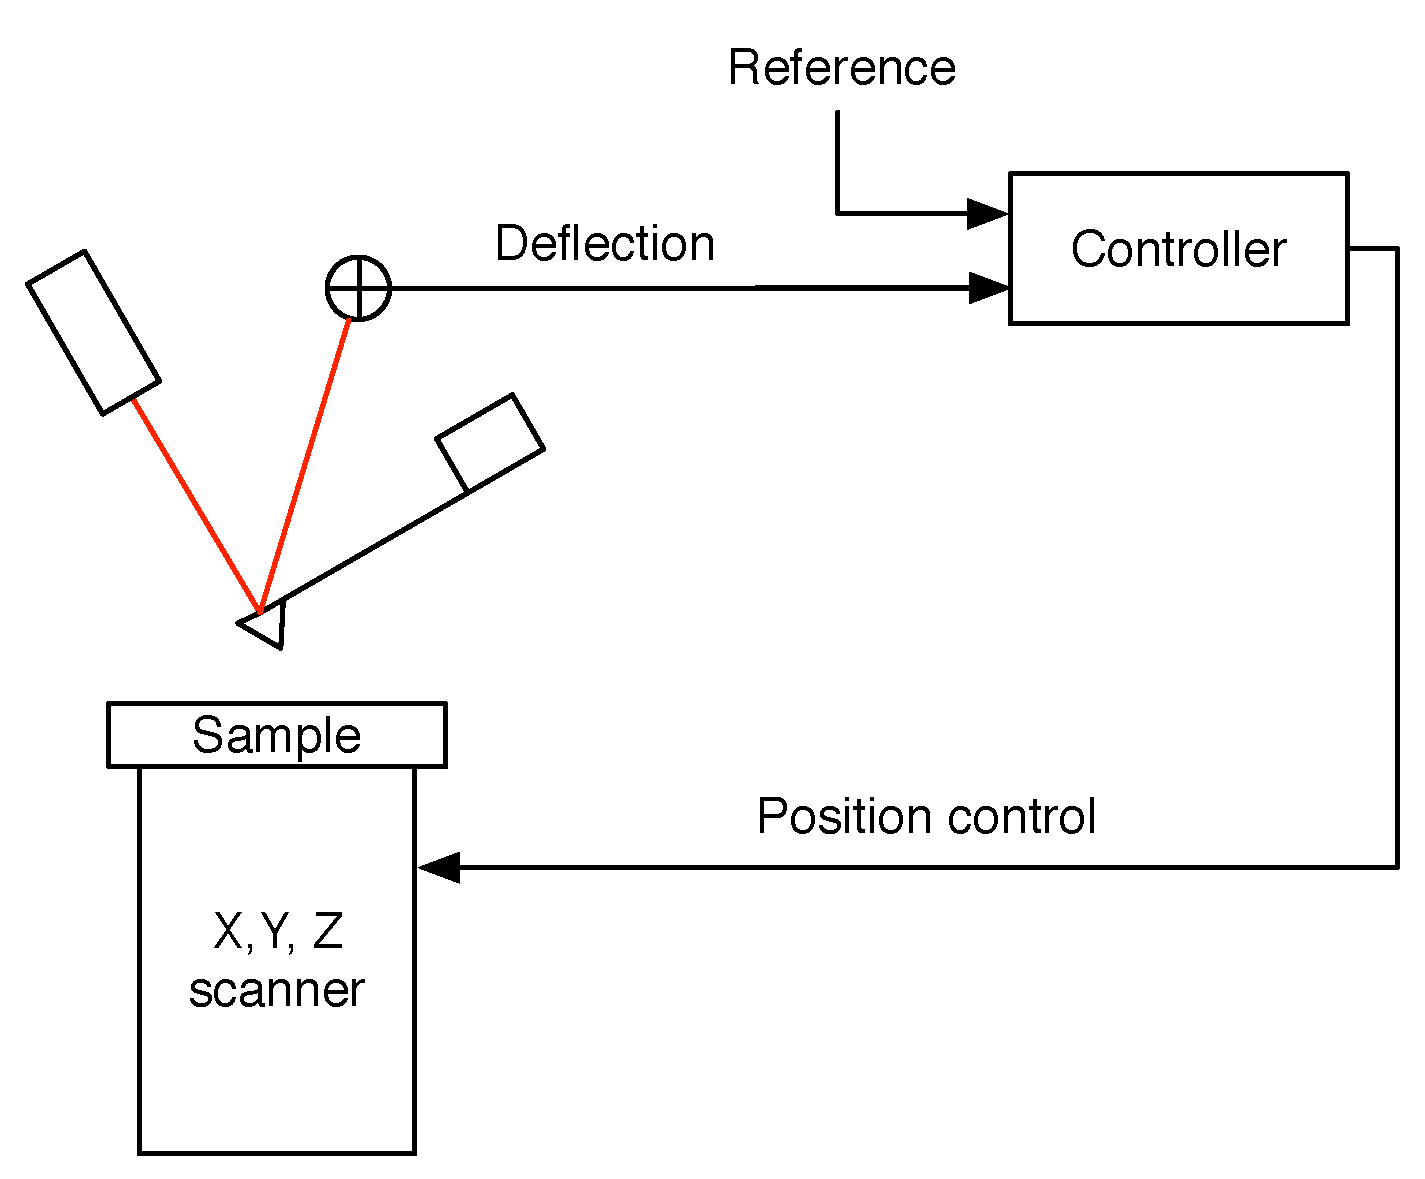
\includegraphics[scale=0.3]{images/normalafm.eps}
    \caption{Normal AFM setup}
  \label{fig:normalAFM}
\end{figure}

The problem with this system is that it can't pick up abrupt changes in the topography.\cite{jeong:093706} The bandwidth of the cantilever is not large enough. This leads to scanning artifacts like parachuting and /ADD OTHER. We could use a cantilever with a higher bandwidth, but the amplitude would be too small. We decided to take to the best of both systems and design a dual-actuator system. We use a standard cantilever to scan the surface and we will add a small piezoelectrical ceramic on top of the X-Y scanner. It enables the AFM to have a larger bandwidth thus allowing it to pick up high spatial frequency topography. 

We design another feedback system in order to make the X,Y,Z scanner and the piezoelectrical ceramic work together. \cite{el2004dual}

\begin{figure}[H]
  \centering
  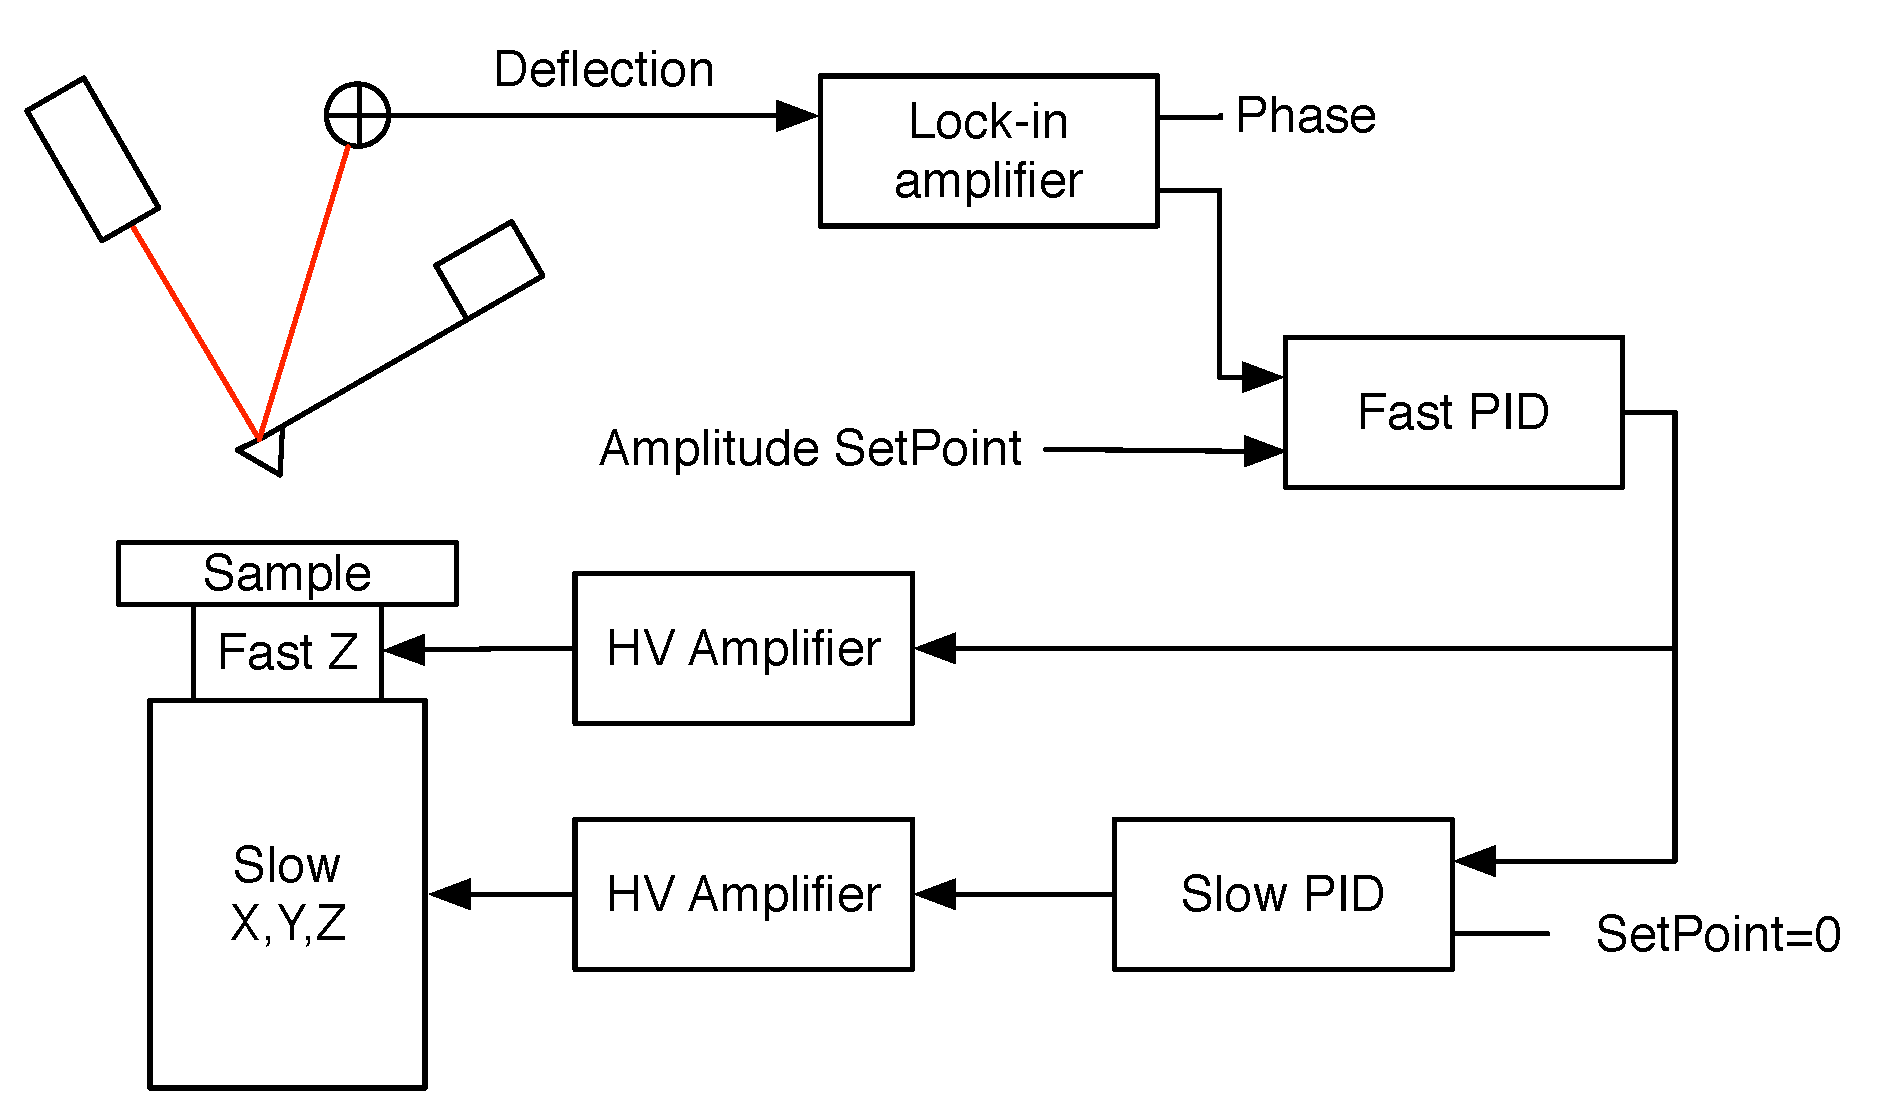
\includegraphics[scale=0.3]{images/doublePID.eps}
    \caption{Z-feedback using fast and slow piezos.}
  \label{DoublePid}
\end{figure}

We need a high-voltage amplifier to operate the small piezoelectric device. 

\section{Tilt compensation}
\label{sec:tiltcompensation}

In theory, the mounted sample should be parallel to the XY-Scanner. If the probe/sample angle is not perpendicular, we observe a tilt on the surface. This tilt is problematic when it becomes larger than the features. There are multiple ways to compensate for this. The most common technique is to use post-processing to adjust the image. Flattening algorithms or first-order planefitting restore the image and put the data on the same level. This technique works if the range of the tip is large enough. We have decided to take another approach and dynamically compensate for the tilt. Before performing our scan, we will do a first scan to compute the tilt of the sample by considering our tilt as a 3D plane. Then, we'll generate a tilt correction signal that will be added to z scan output.

We use a circle pattern to scan the surface of the sample. The radius of the circle is equal to the scan size. It gives us information about the general topography of the surface. Then, we compute the plane equation of the surface by applying a fit in Igor Pro. This fit will generate a plane that models the tilted surface. The input of this fit is the theoretical X-Y output waves of the circle pattern: a sine and a cosine. The data on the z axis is the height.

\begin{equation}\label{eqn:planeeq}
z = a_1 x + a_2 y + a_3 
\end{equation}

The coefficients are computed by minimizing the values of Chi-Square (error function). Then, we generate the waves to send to the controller with the equation ref.

\begin{equation}\label{eqn:sendwave}
wavetosend = a_1 wavex + a_2 wavey 
\end{equation}

Wavex and wavey are the output of our scan pattern. With this method, we can do a tilt correction with any scan pattern.

Then, we send the previously computed wave to the controller.

\begin{figure}[H]
  \centering
  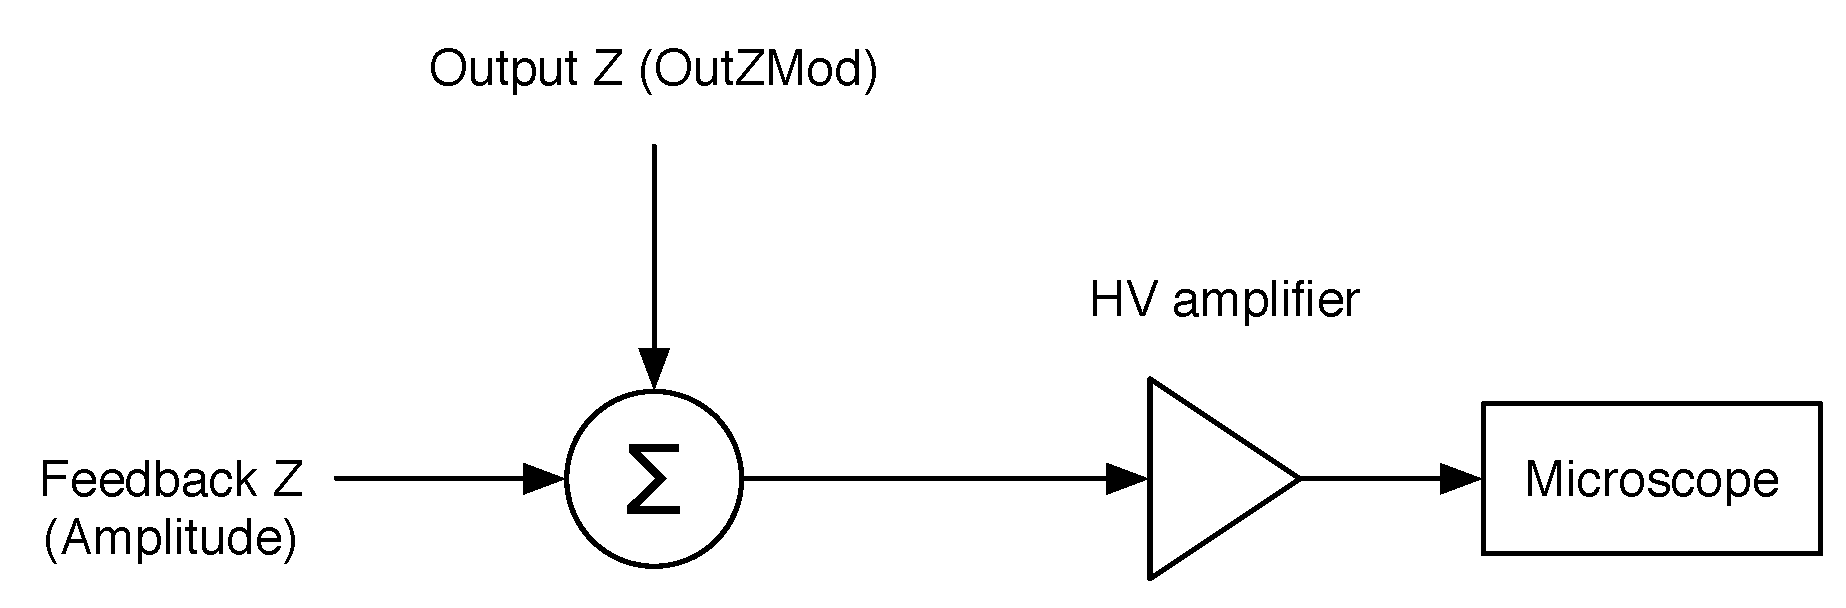
\includegraphics[scale=0.4]{images/outputz.eps}
    \caption{Asylum}
  \label{outputz}
\end{figure}